%% TIPO DE DOCUMENTO 

\documentclass{beamer}

\usetheme{Madrid}
\usecolortheme{seagull}
\usefonttheme{professionalfonts}

%%% IMPORTAMOS PAQUETES A USAR 

\usepackage[utf8]{inputenc}
%\usepackage[latin1]{inputenc}
\usepackage[spanish, es-tabla]{babel}
\usepackage{csquotes}
\usepackage{float}
\usepackage{graphicx}
\usepackage{hyperref}
%Pruebas para animaciones
\usepackage{animate}
\usepackage[document]{ragged2e}
\usepackage{bibentry}
\usepackage{graphicx} % Allows including images
\usepackage{booktabs} % Allows the use of \toprule, 

%%%START APA
%\usepackage[british]{babel}
%\usepackage[backend=biber,style=apa]{biblatex} OJO CON ESTA LINEA
\setbeamertemplate{navigation symbols}{} % To remove the navigation symbols from the bottom of all slides uncomment this line
%\DeclareLanguageMapping{british}{british-apa}
%\addbibresource{references.bib}
%% APA citing
%% \cite{t} - Uthor und Richter, 2010
%% \textcite{t} - Uthor und Riter (2010)
%% \parencite{t} - (Uthor & Riter, 2010)
%% \parencite[Chapt.~4]{t} - (Uthor & Riter, 2010, S. 15)
%%%END APA

%%%%% =================  PORTADA ================== 

\title[Universo Medible II] 
{Universo Medible II \\ Astronomía de posición}
%\subtitle {ne compléter que si l'article possède un sous-titre}

\author[Victor M. Santos] 
%\author[Pedro A. Salgado-Meza ]
{Victor M. Santos \inst{} \and M.Tarazona-Alvarado \inst{} \and J. Pisco-Guabave \inst{}} %\inst{1} \inst{3}}
%{P. A. ~Salgado-Meza\inst{1} \inst{2}}%\and I.~Borne\inst{1} \and J.~Buisson\inst{2}}

\institute[]{
\inst{}Grupo Halley, Escuela de Física, Universidad Industrial de Santander, Bucaramanga, Colombia.}
%\institute[]
%{
%  \inst{1}%
%  Universidad Industrial de Santander, Bucaramanga, Colombia
%  \and
%  \inst{2}%
%  Escuela de Ingenierías Eléctrica, Electrónica y Telecomunicaciones
%  \and
%  \inst{3}%
%  Escuela de Ingeniería Mecánica  
%  }

\date{\today}


\begin{document}
\logo{
\includegraphics[scale=0.3]{Imagenes/Logo_Halley}} 


\begin{frame}{Grupo Halley}
\titlepage % Print the title page as the first slide
\end{frame}

%%%%%%%%%%%%%%%%%%%%%%%%%%%%%%%%%%%%%%%%%%%%%%%%%%%%%%%%%%%%%%%%%%%%%%%%%%%%%%%%%%%%%%%%%

\begin{frame}
 \begin{columns}
 \column{.45\textwidth}
  \begin{figure}
   \centering
   %\raggedright
   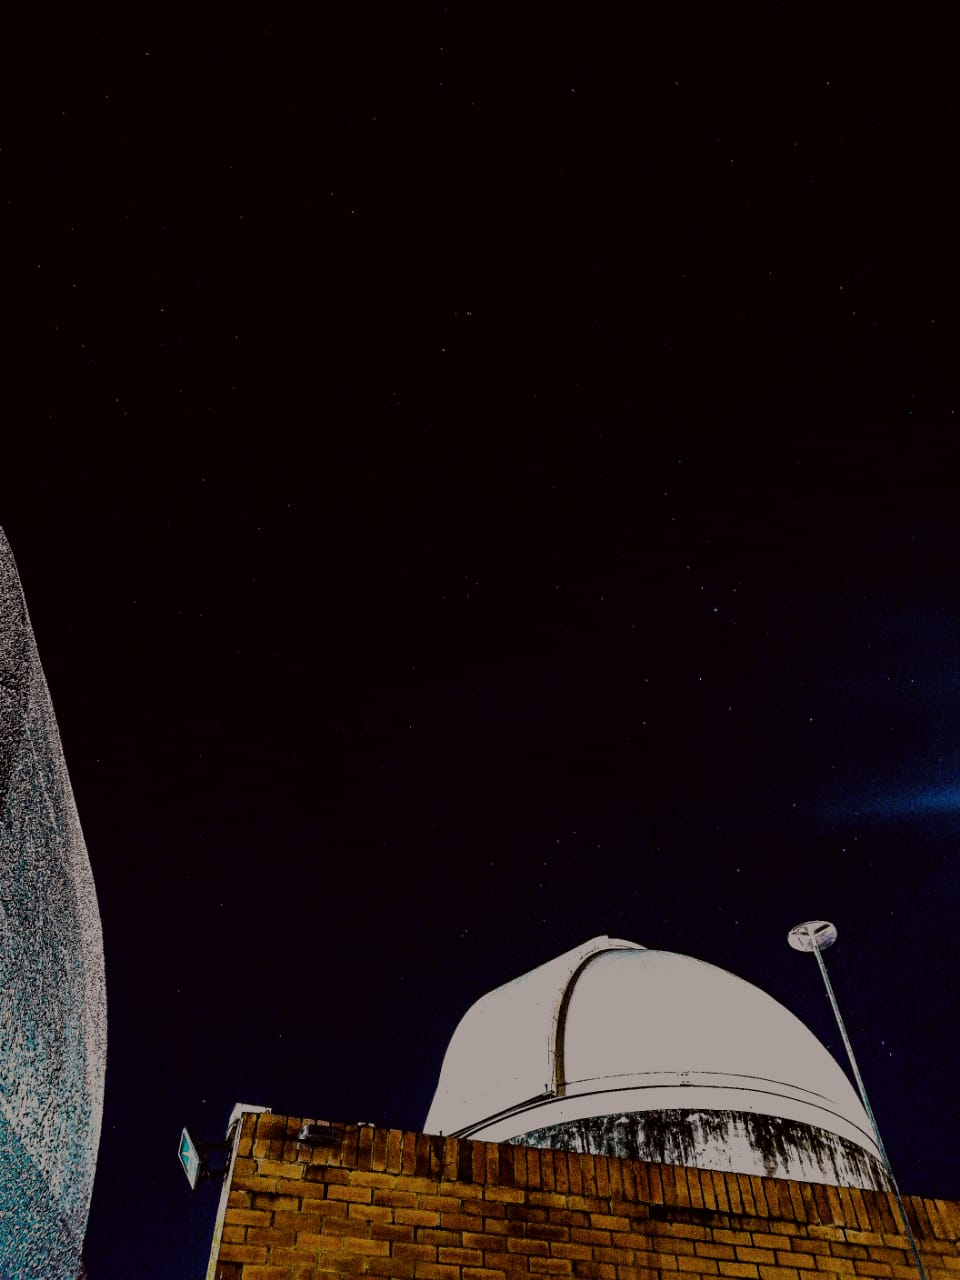
\includegraphics[scale=0.15]{Imagenes/Halley}
  \end{figure}
 \column{.45\textwidth}
 \small
 \justify
  El \textbf{Grupo Halley} se ha caracterizado por ser líder en divulgación de astronomía en el nororiente colombiano. Los programas de extensión son parte fundamental de la misión del grupo Halley, ya que facilita establecer vínculos con la comunidad mientras se construye una cultura científica y crítica.
 \end{columns}
\end{frame}

%%%%%%%%%%%%%%%%%%%%%%%%%%%%%%%%%%%%%%%%%%%%%%%%%%%%%%%%%%%%%%%%%%%%%%%%%%%%%%%%%%%%%%%

\begin{frame}{Universo Medible II}
 \begin{columns}
 \column{.45\textwidth}
  \begin{figure}
   \centering
   %\raggedright
   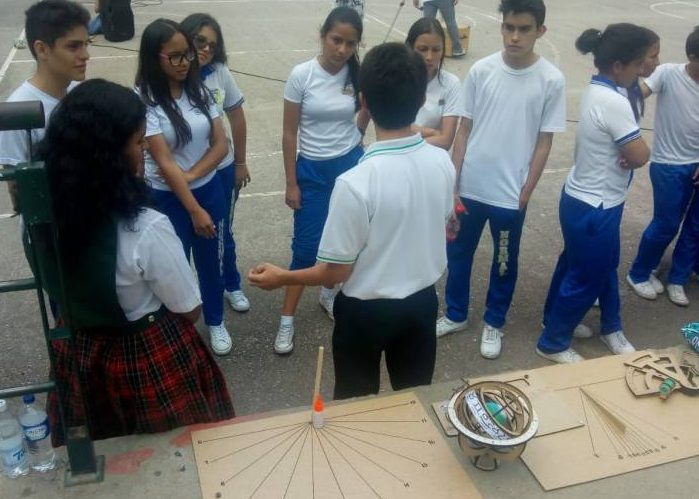
\includegraphics[scale=0.2]{Imagenes/UM_02}
  \end{figure}
  \begin{center}
  \Tiny
  Divulgación en el parque de los niños - 2018
  \end{center}
 \column{.45\textwidth}
 \small
 \justify
  Universo Medible II exhibe una alternativa de aprendizaje de astronomía de posición. Se desarrolla con estudiantes de educación media, quienes utilizan instrumentos clásicos junto a herramientas computacionales  durante su proceso de aprendizaje. Finalmente se comparten los conocimientos adquiridos en ambientes divulgativos contribuyendo al desarrollo de una cultura científica.
 \end{columns}
\end{frame}
%%%%%%%%%%%%%%%%%%%%%%%%%%%%%%%%%%%%%%%%%%%%%%%%%%%%%%%%%%%%%%%%%%%%%%%%%%%%%%%%%%%%%%%%%%%%%%%%%%%%%%%%%%%%%%%%%%%%%%%%


\begin{frame}{Generalidades}
\begin{itemize}
\item Sesiones $\rightarrow$ 16 sesiones (cuatro meses)
\item Tiempo por sesión $\rightarrow$ dos horas
\item Instrumentos
\item Python 
\item Contenido
 \begin{itemize}
  \item Distancias astronómicas
  \item Movimientos de la Tierra
  \item Solsticio y equinoccio
  \item Constelaciones
  \item Propiedades de la luz
  \item Coordenadas 
 \end{itemize}
\end{itemize}
\end{frame}

%%%%%%%%%%%%%%%%%%%%%%%%%%%%%%%%%%%%%%%%%%%%%%%%%%%%%%%%%%%%%%%%%%%%%%%%%%%%%%%%%%%%%%%%%%%%%%%%%%%%%%%%%%%%%%%%%%%%%%%

\begin{frame}
\begin{center}
\Huge 
\textit{``La ciencia más útil es aquella cuyo fruto es el más comunicable."}
\end{center}
\begin{flushright}
\small
\textit{Leonardo Da Vinci}
\end{flushright}


\end{frame}
\end{document}